%-----------------------------------LICENSE------------------------------------%
%   This file is part of Mathematics-and-Physics.                              %
%                                                                              %
%   Mathematics-and-Physics is free software: you can redistribute it and/or   %
%   modify it it under the terms of the GNU General Public License as          %
%   published by the Free Software Foundation, either version 3 of the         %
%   License, or (at your option) any later version.                            %
%                                                                              %
%   Mathematics-and-Physics is distributed in the hope that it will be useful, %
%   but WITHOUT ANY WARRANTY; without even the implied warranty of             %
%   MERCHANTABILITY or FITNESS FOR A PARTICULAR PURPOSE.  See the              %
%   GNU General Public License for more details.                               %
%                                                                              %
%   You should have received a copy of the GNU General Public License along    %
%   with Mathematics-and-Physics.  If not, see <https://www.gnu.org/licenses/>.%
%------------------------------------------------------------------------------%

%   Use the standalone class for displaying the tikz image on a small PDF.
\documentclass[crop, tikz]{standalone}

%   Import the tikz and pgfplots packages to use for the drawing.
\usepackage{tikz, pgfplots}

%   Load the arrows.meta and calc library.
\usetikzlibrary{arrows.meta, calc}

%   Begin the document.
\begin{document}
    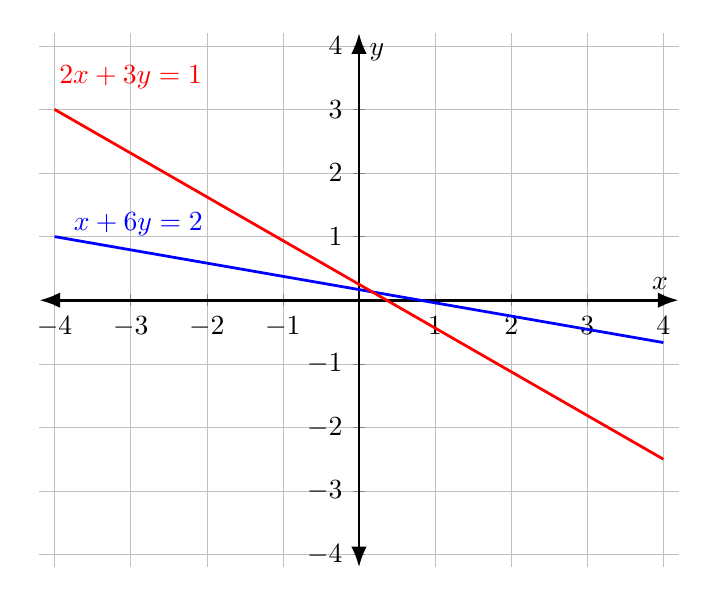
\begin{tikzpicture}[>=Latex]

        %   Use the axis environment to draw a grid and axes.
        \begin{axis}[%
            width=0.8\linewidth,
            axis lines=center,
            axis line style={<->},
            xtick distance=1,
            xlabel=$x$,
            xmin=-4.2,
            xmax=4.2,
            ytick distance=1,
            ylabel=$y$,
            ymin=-4.2,
            ymax=4.2,
            grid=both,
            grid style={line width=.1pt, draw=gray!10},
            major grid style={line width=.2pt,draw=gray!50},
            line width=1pt
        ]

            %   Draw the two lines representing the equations.
            \draw[draw=blue] (axis cs:-4.0, 1.0) to (axis cs:4.0, -0.666);
            \draw[draw=red] (axis cs:-4.0, 3.0) to (axis cs:4.0, -2.5);

            %   Label everything.
            \node at (axis cs:-2.9, 1.2) {$\color{blue}x+6y=2$};
            \node at (axis cs:-3.0, 3.5) {$\color{red}2x+3y=1$};
        \end{axis}
    \end{tikzpicture}
\end{document}
